% !TeX root = ./DLVCQuestions.tex
\section{Image classification}
\subsection{What is the task definition of image classification?}
Predict the label (picked from a set of possible labels) of an image, i.e.: what is visible on the image. Output could also be a distribution over labels to indicate confidence in result.

\subsection{Explain at least 5 challenges and give examples.}
\begin{itemize}
\item Viewpoint variation: A single instance of an object can be oriented in many ways with respect to the camera.
\item Scale variation: Visual classes often exhibit variation in their size (size in the real world, not only in terms of their extent in the image).
\item Deformation: Many objects of interest are not rigid bodies and can be deformed in extreme ways, e.g. water
\item Occlusion: Only a small portion of an object (as little as few pixels) could be visible.
\item Illumination conditions: The effects of illumination are drastic on the pixel level.
\item Background clutter: The objects of interest may blend into their environment, making them hard to identify.
\item Intra-class variation: The classes of interest can often be relatively broad, such as chair. There are many different types of these objects, each with their own appearance.
\item Abstraction (human able to recognize some doodle as the correct object usually---difficult to recognize for machines as e.g. difference between cow and dog in a doodle may be the presence of grass
\item Invariants (an object may be the same object if it's rotated by some degree. Other objects (e.g. ``6'' and ``9'') are not invariant under rotation
\end{itemize}

\subsection{What is object detection and how does it differ from classification?}
Object detection tries to find all objects present in an image whereas in image classification a label is assigned to the whole image. Object detection can be reduced to image classification (classify various parts of the image and combine results)

\section{Datasets}

\subsection{Why do we need datasets?}Data required for training and testing of model. 
	
\subsection{What are the challenges of dataset collection and annotation in deep learning?}Datasets should be sampled from the same distribution as images which are then classified, i.e. it should span the whole space of possible features associated with each class. For example if dataset contains only cats run over by car a model trained with this set will have difficulties recognizing healthy cats.

\subsection{Explain the purpose of the different subsets.}
\begin{itemize}
\item Training set: Used to train the model
\item Validation set: Used to train hyperparameters
\item Test set: Final performance analysis. 
\end{itemize}
Model is trained with training set and then evaluated with validation set. Then some other hyperparameters are chosen (e.g. lower learning rate, \ldots) and the step is repeated until there is no further improvement to the model. The datasets have to be disjunct as else it would be ``learning to the test'' (e.g. model is a hashmap containing the hash of the image and the correct class. Would work if testset is contained in training set but completely useless for new data)

\subsection{What is the rule of thumb about how many images per classes are needed for CNNs to perform well?}
Approximately 1000 per class---more usually does not hurt though.


\section{Case study}

\begin{quote}
Assume a company asks you to develop an application that is able to predict which kind of bird is depicted in a given image. List and explain the individual steps you’d follow to solve this problem using deep learning.
\end{quote}
\begin{enumerate}
\item (Set up some machine that allows to train the model with hardware acceleration)
\item Ask what kind of birds should be distinguished from each other (e.g. is ``parrot'' enough or should it be ``macaw parrot'' or even ``Ara'' or ``Military macaw'')
\item Only sitting birds or also while they're flying? 
\item Look for dataset that fulfills the conditions resulting from the above questions
\item Proceed in the usual order to train a model:
\begin{itemize}
\item Set up training process
\item Find suitable NN architecture
\item Augment dataset 
\item Find hyperparameters and tune them until accuracy is good enough
\end{itemize}
\end{enumerate}

%: DL Motivation
%: Classification \& Regression/ Supervised vs unsupervised learning
%: Testdata
%: Performance measures
%: Capacity, bias, variance
\section{Hyperparameter}
\subsection{What is a hyperparameter?}
In ML we try to find parameters for a model from datasets. This learning process may have its own parameters, these are called hyperparameters. They govern behaviour of the model learning, .e.g. the capacity of the resulting model.
\subsection{Name at least 3 hyperparameters in the context of deep learning using convolutional neural networks.}
\todo{maybe explain what these hyperparameters do}
\begin{enumerate}
\item Initial learning rate
\item Learning rate decay
\item Regularization strength
\item Momentum settings
\end{enumerate}
\subsection{What is the purpose of hyperparameter selection, which search strategies exist, and how do they work?}
Purpose is finding optimal settings to train the model. Gridsearch and random search are two common approaches, random search is usually preferred as one parameter may be insignificant for the result and much time would be wasted optimizing this parameter whereas with random search all HP spaces are explored independently. See picture below.

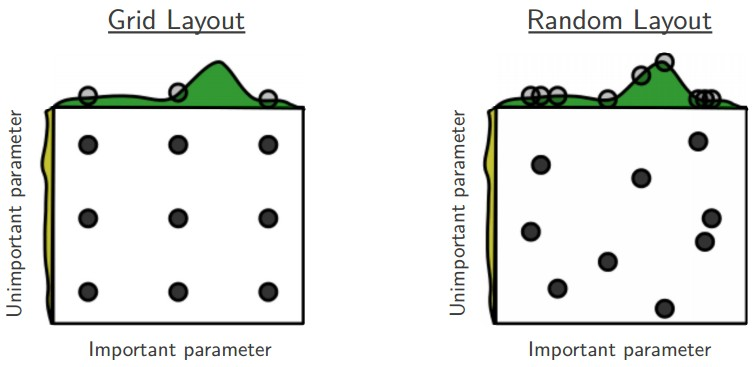
\includegraphics[width=\textwidth]{./img/gridsearchbad.jpeg}


\section{kNN}
\subsection{How does the k nearest neighbor classifier work?}
Find the k samples in the training set that are most similar to the current sample according to some similarity measure

\begin{itemize}
\item Training
\begin{itemize}
\item Preprocess data 
\item Transform images to vectors ($32\times 32\times 3 \text{ image }\to 32\cdot 32\cdot 3 = 3072$D vector) or use extracted feature vector
\item Split into training and validation data and optimize the hyperparameters (distance measure and $k$)
\end{itemize}
\item Classification
\begin{itemize}
\item Apply the same preprocessing  transformations as before
\item Find the k images that are most similar and use the most common label as prediction (or output the distribution of labels)
\end{itemize}
\end{itemize}

\subsection{Sketch of kNN}
\begin{minipage}{0.65\textwidth}
{Create a sketch for illustration, assuming a two-dimensional feature space and two different classes, Draw at least three training samples per class (must not lie on a line) as well as (roughly) the resulting decision boundaries.}

Image on right is kNN with two classes and $k=1$.
\end{minipage}
\begin{minipage}{0.4\textwidth}

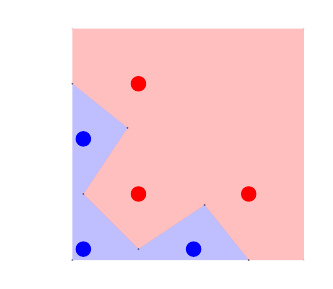
\begin{tikzpicture}[scale=1.4]
\draw[white] (-0.5,-0.1) rectangle(2,2);
\fill[blue] (0,0)circle(2pt);
\fill[blue] (1,0)circle(2pt);
\fill[blue] (0,1)circle(2pt);
\fill[red] (0.5,0.5)circle(2pt);
\fill[red] (1.5,0.5)circle(2pt);
\fill[red] (0.5,1.5)circle(2pt);
\def\pointset{(-0.1,1.5),(0.4,1.1),(0,0.5),(0.5,0),(1.1,0.4),(1.5,-0.1),(2,-0.1),(2,2),(-0.1,2)}
\foreach \x[count=\i] in \pointset
  \fill [opacity=0.1] \x circle(0.25pt) coordinate (mark-\i);
\fill [opacity=0.25,red]
  (mark-1) \foreach \x[count=\i] in \pointset{ -- (mark-\i) } -- cycle;

\def\pointset{(-0.1,1.5),(0.4,1.1),(0,0.5),(0.5,0),(1.1,0.4),(1.5,-0.1),(-0.1,-0.1)}
\foreach \x[count=\i] in \pointset
  \fill [opacity=0.5] \x circle(0.25pt) coordinate (mark-\i);
\fill [opacity=0.25,blue]
  (mark-1) \foreach \x[count=\i] in \pointset{ -- (mark-\i) } -- cycle;
\end{tikzpicture}
\end{minipage}
\subsection{What are the limitations of this classifier?}
\begin{itemize}
\item Classification performance is rather bad as sample has to be compared to all/most of the samples in the training set (can be improved with KDTree from $O(n)$ to $O(log(n)^d)$ or similar)
\item Does not recognize higher order features, e.g. ``presence of wheels'' but only uses similarity of features (pixels). Completely thrown off the track by e.g. different lighting or position of object in image (e.g. off center in sample and only centered pictures in training set)
\item Very sensitive to background
\end{itemize}

%: Image Classification
%: Parametric model
%: Linear model
%: Loss function
%: Optimization in ML
\section{Local/global optimum}
\subsection{What is the difference between a local and a global optimum?}
A function has only one global optimum but may have many local optima. Finding the global optimum is not trivial whereas finding a local optimum is usually easy (calculate derivation at current point and move in direction of steepest descent). When a local optimum is found it's nontrivial how to escape it again. Simulated annealing is an approach inspired from material physics.

\includegraphics[width=\textwidth]{./img/localopt.jpeg}
\subsection{Are local minima a problem in deep learning?  Why (not)?}
There is no definite consensus though it is believed, that the search landscape is similar to an egg carton with many almost identical local optima where the hit on the performance is not critical if the model finds any of them. It was also proposed that many local optima (as found by having a derivation of 0) in the search landscape are in reality saddle points where it should be possible to improve the results further. Calculating the full Hessian is too costly therefore an approximation may be enough. (see here: \url{https://blog.terminal.com/no-more-local-minima/})
%: Gradient descent
%: Batch Gradient descent
%: Weight and bias parameters
%: Preprocessing
%: Optimization vs ML
%: Regularization
%: Feedforward NN
%: MLP
%: MLP for VC
%: Representation learning
%: Locally connected layers for image analysis
%: Conv Layer
%: Receptive field
\section{Pooling}
\subsection{What is the purpose of pooling layers?}
Reduce spatial size to reduce amount of parameters and computation. Also helps against overfitting. Consolidate features learned in convolutional layers before the pooling layer.
\subsection{Calculate the output of a 2 × 2 max-pooling layer with stride 2 assuming the following input.}
\begin{equation}
pool\left(\begin{bmatrix}
1 & 1 & 2 & 4\\
5&6&7&8\\
3&2&1&0\\
1&2&3&4
\end{bmatrix}\right) = \begin{bmatrix}6 & 8 \\3 & 4\end{bmatrix}
\end{equation}
\subsection{How many pooling layers with stride 2 should a CNN have assuming an input resolution of 64 × 64 and convolutional layers that do not change the resolution, and why?}
\todo{How many pooling layers should CNN have?}
%: CNN
%: CNN depth
%: CNN backend
%: ResNets
\section{Back Propagation}
\subsection{What is the purpose of the backpropagation algorithm?}
\begin{itemize}
\item { Compute gradient of computation graph given by NN and current parameters}
\item { Starting from input calculate derivatives of all nodes by their children. Sum up derivatives multiplied over all paths from output to input node to get derivation of output by input node. }
\item { Gets inefficient really fast if multiple paths from input to output exist. Reverse accumulation strategies help in this case (reverse mode differentation)}
\end{itemize}
\subsection{Example}
\begin{quote}
{Assume the following computational graph. Insert digits from your Matrikelnummer into the empty input nodes, going from right to left both in terms of nodes and digits. Then compute the partial derivative of the topmost node with respect to all input nodes via  backpropagation. Write computation node values after the forward pass left of the nodes, local gradients left of the edge connecting the corresponding nodes, and “cached” partial derivatives of the topmost node right to the nodes.}
\end{quote}
\tikzset{
  treenode/.style = {align=center, inner sep=0pt, text centered,font=\sffamily},
  calc/.style = {treenode, circle, draw=black, black,fill=green!25, text width=1.5em},
  numbr/.style = {treenode, circle, draw=black, black,fill=red!25, text width=1.5em},
  input/.style = {treenode, circle, draw=black, black,fill=blue!25, text width=1.5em},
}
\begin{minipage}{0.7\textwidth}
\begin{tikzpicture}[->,>=stealth',level/.style={sibling distance = 5cm/#1,
  level distance = 1.5cm}] 
\node [calc] {* 455}
    child{ node [calc] {+ 35} 
            child{ node [numbr] {5}  edge from parent node[above left]{$1$}}
            child{ node [calc] {* 30 } 
		child{ node [input] {5}edge from parent node[left]{$5$}}
		child{ node [input] {6} coordinate (AA) edge from parent node[right]{$6$}}
		edge from parent node[above right]{$1$}
            }            edge from parent node[above]{$13$}                
    }
            	child{ node [calc] {+ 13}   coordinate (BB)
			child{ node [input] {7}edge from parent node[below right]{$1$}}
			edge from parent node[right]{$35$}
	            }    
; 
\draw[->,>=stealth']( $ (BB)!15pt!(AA) $ )--( $ (AA)!10pt!(BB) $ );
\end{tikzpicture}
\end{minipage}\begin{minipage}{0.3\textwidth}
\begin{align*}
\partial a &= 13\cdot 1 \cdot 5 = 65\\
\partial b &=  13\cdot 1 \cdot 6 + 35\cdot 1 = 113\\
\partial c &= 35 \cdot 1 = 35
\end{align*}
\end{minipage}
\subsection{Explain the steps of the algorithm at a given node.}
\begin{itemize}
\item { First calculate values at every node}
\item{ Then derive each node by input parameters to get partial derivatives}
\item{ Multiply every path from an input to output (chain rule $g(f)' = g'(f)\cdot f'$}
\item { Sum up all paths from input to output (product rule: $(g\cdot f)' = g'\cdot f + f'\cdot g$}
\end{itemize}
%: Data Agumentation
%: Dropout
%: Batch normalization
\section{Learning rate}
\subsection{What does the learning rate hyperparameter specify?}
The direction of steepest decrease can be calculated with the gradient, the size of the optimal stepsize is unknown and instead the stepsize given by the learning rate hyperparameter is used. The choice of this parameter is critical. 

If learning rate is:
\begin{itemize}
\item very high: Gradient descent algorithm jumps over minima and is more or less a random walk in configuration space
\item high: Finds a better configuration then the random starting configuration but gets stuck there as it ``oscillates'' around minimum (e.g. minimum is in a circle with radius 2 and algorithm makes steps with size 5
\end{itemize}
\begin{minipage}{0.6\textwidth}
\begin{itemize}
\item properly: First missclassification rate quickly decreases and then slowly converges to some minimum
\item low: Finds minimum as well but very slow (progress looks linear whereas in the beginning almost exponential decay of error should be possible)
\end{itemize}
\end{minipage}\begin{minipage}{0.4\textwidth}
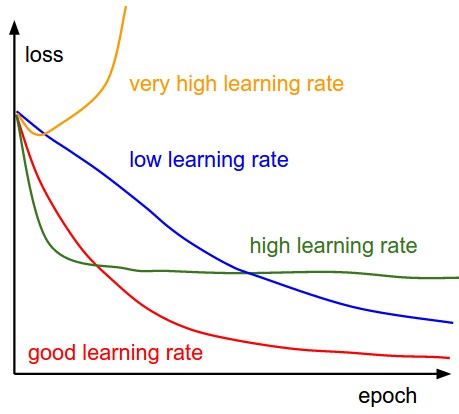
\includegraphics[width=\textwidth]{./img/learningRate.jpeg}
\end{minipage}
\subsection{Explain a heuristic for adapting the learning rate during training and why doing can be beneficial.}
Learning rate decay can be used to tune the learning rate to the optimal choice at each step. First start with a rather high learning rate and when there is no improvement for a few epochs scale the learning rate with a constant factor (e.g. $\nicefrac 1 2$).
Alternatively scale the learning rate every 5-20 epochs with a factor ($\nicefrac 1 2$ to $\nicefrac 1 {10}$). This ensures that big steps are taken by the algorithm when it is possible but the stepsize is reduced when further improvements can only be made by smaller steps.

%: Oversampling
%: Model ensembles
%: Model ensembles
%: Medical tasks
%: 2-3D deep CNN
%: ??
%: CNNs in medical imaging
%: Labelling
%: RNNs
%: LSTMs